% Chapter 3

\chapter{Circuit Diagram and Calculation} % Write in your own chapter title
\label{Chapter2}
\lhead{Chapter 3. \emph{Circuit Diagram and Calculation}} % Write in your own chapter title to set the page header
 \section{Shematic}
 Below is the shematic of 555 Sampler that is simulated on proteus.
 	\begin{figure}[htbp]
	\centering
	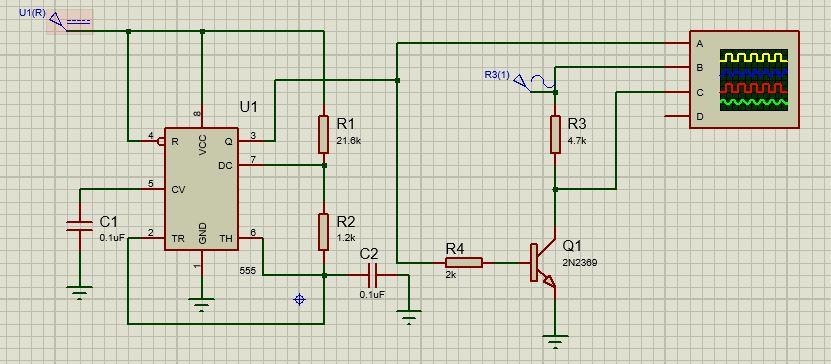
\includegraphics[width = 4in]{./Figures/schematic.jpg}
	\rule{35em}{0.5pt}
	\caption{schematic}
\end{figure}

 \section{calculation}
 \subsection{Different R value combinations at 95\%}
 frequency calculation:
   \[f_s = \frac{1}{T}=\frac{1.44}{(R_1 + 2R_2)C_1} \]
 Duty cycle calculation:
    \[D = \frac{R_2}{R_1+2R_2} \]
High and Low Time
    \[T_H=0.7(R_1 + R_2) C_1\] 
    \[T_L=0.7*R_2*C_1\] 
 \begin{center}
 \begin{tabular}{ |p{3cm}|p{3cm}|p{3cm}|  }
 	\hline
 	\multicolumn{3}{|c|}{Input parameters} \\
 	\hline
 	Capacitance C_1& Value of Resistance R_1 &Value of Resistance R_2\\
 	\hline
 	0.1uF & 3.24$k\Omega$ & 180$\Omega$\\
 	\hline
 \end{tabular}
 \end{center}
  \begin{center}
 \begin{tabular}{ |p{3cm}|p{3cm}|p{3cm}|p{3cm}| }
 	\hline
 	\multicolumn{4}{|c|}{Output parameters} \\
 	\hline
 	Frequency& Time period &High time & Low Time\\
 	\hline
 	4 kHz & 25 millisecond & 23.94 millisecond& 126 millisecond\\
 	\hline
 \end{tabular}
 \end{center}
 	\begin{figure}[htbp]
	\centering
	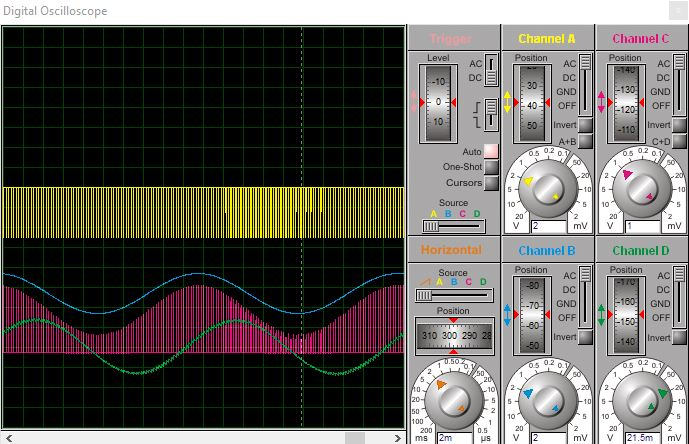
\includegraphics[width = 4in]{./Figures/1.jpg}
	\rule{35em}{0.5pt}
	\caption{schematic}
\end{figure}
	
\begin{center}
 \begin{tabular}{ |p{3cm}|p{3cm}|p{3cm}|  }
 	\hline
 	\multicolumn{3}{|c|}{Input parameters} \\
 	\hline
 	Capacitance C_1& Value of Resistance R_1 &Value of Resistance R_2\\
 	\hline
 	0.1uF & 8.46$k\Omega$ & 470$\Omega$\\
 	\hline
 \end{tabular}
 \end{center}
  \begin{center}
 \begin{tabular}{ |p{3cm}|p{3cm}|p{3cm}|p{3cm}| }
 	\hline
 	\multicolumn{4}{|c|}{Output parameters} \\
 	\hline
 	Frequency& Time period &High time & Low Time\\
 	\hline
 	1531.9 Hz & 65.28 millisecond & 62.51 millisecond& 329 millisecond\\
 	\hline
 \end{tabular}
 \end{center}
 	\begin{figure}[htbp]
	\centering
	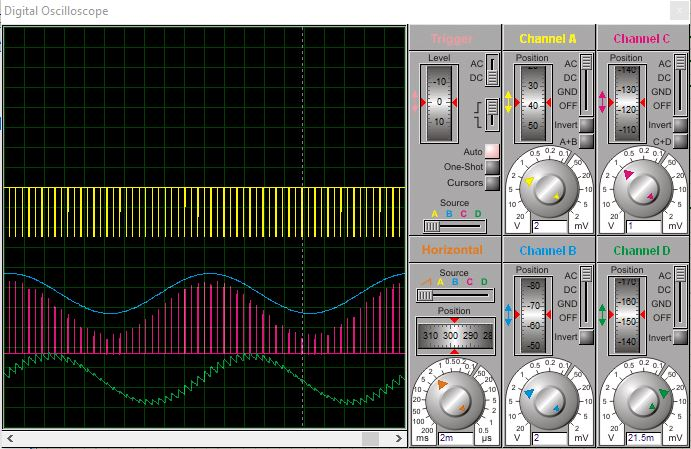
\includegraphics[width = 4in]{./Figures/2.jpg}
	\rule{35em}{0.5pt}
	\caption{schematic}
\end{figure}
\section{Design of filter}
As we know that 
  \[RC < \frac{1}{2} \]
  \begin{figure}[htbp]
	\centering
	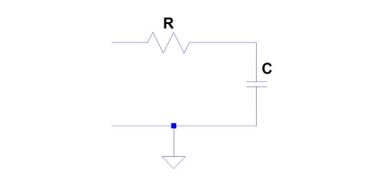
\includegraphics[width = 4in]{./Figures/filter.jpg}
	\rule{35em}{0.5pt}
	\caption{Low pass RC filter}
\end{figure}
\\Value of Resistance R_1 = \underline{3240$\Omega$} 
\\Value of Resistance R_2 = \underline{180$\omega$} 
\\sampling frequency = \underline{4000kHz} 
\\Resistanc value = \underline{8$k\Omega$} 
\\Capacitance = \underline{1uF} 
	\begin{figure}[htbp]
	\centering
	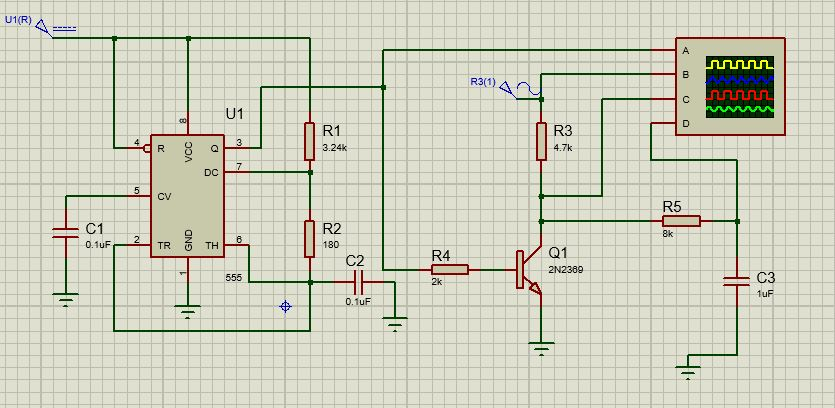
\includegraphics[width = 4in]{./Figures/schematic1.jpg}
	\rule{35em}{0.5pt}
	\caption{sampling at 4000 Hz}
\end{figure}

\\Value of Resistance R_1 = \underline{3240$\Omega$} 
\\Value of Resistance R_2 = \underline{180$\omega$} 
\\sampling frequency = \underline{4000kHz} 
\\Resistanc value = \underline{8$k\Omega$} 
\\Capacitance = \underline{1uF} 
	\begin{figure}[htbp]
	\centering
	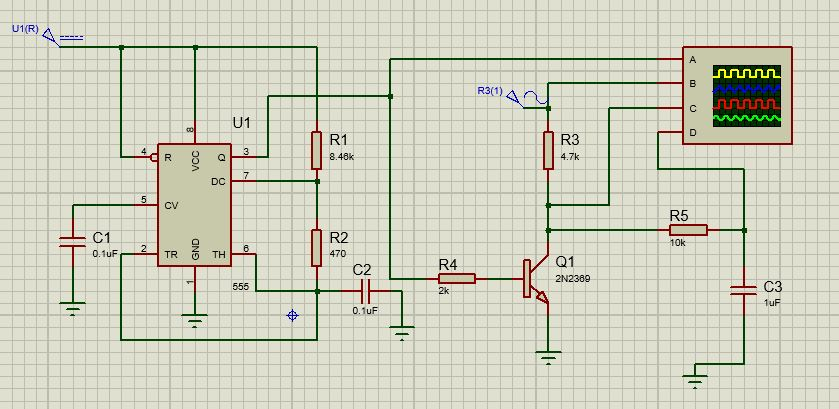
\includegraphics[width = 4in]{./Figures/schematic2.jpg}
	\rule{35em}{0.5pt}
	\caption{sampling at 1531 Hz}
\end{figure}